% The two declared task-boundary differences, stated as certificate tests.
% Each panel pairs the rendered structure with the two contracts that disagree
% and with the mirror-certificate comparison that decides the exact verdict.
% Requires concept_style.tex; libraries arrows.meta, calc, backgrounds.
\begin{tikzpicture}[
  font=\small,
  chip/.style={rounded corners=2pt, line width=0.5pt, font=\scriptsize,
    inner xsep=3.6pt, inner ysep=2.4pt},
  acs/.style={chip, draw=black!32, fill=black!2, text=black!62},
  chiral/.style={chip, draw=ioBlue!60!black, fill=ioBlue!8,
    text=ioBlue!42!black, font=\scriptsize\bfseries},
  achiral/.style={chip, draw=ioGreen!62!black, fill=ioGreen!10,
    text=ioGreen!42!black, font=\scriptsize\bfseries},
  crit/.style={font=\scriptsize, text=black!70},
  why/.style={font=\scriptsize, text=black!58, align=center,
    text width=6.25cm, inner sep=0pt},
]

% ------------------------------- A: VS170 --------------------------------
\begin{scope}
  \filldraw[iopanel] (-7.25,-0.78) rectangle (-0.15,5.60);
  \node at (-3.70,2.75)
    {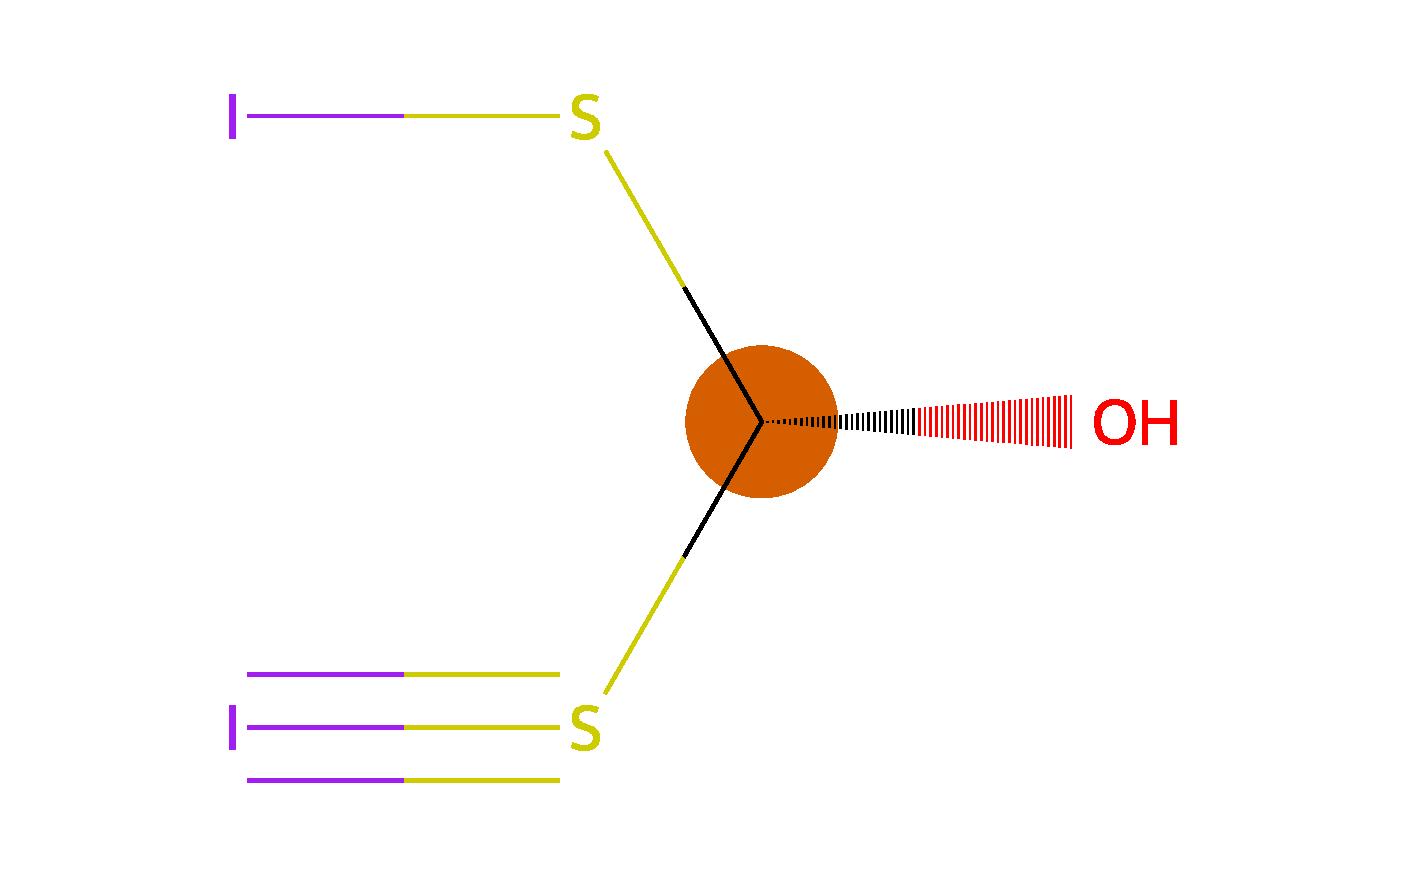
\includegraphics[width=6.0cm]{fig/exact_mirror_vs170.pdf}};
  \iosub{-6.92,5.26}{A}{VS170}
  \node[acs,     anchor=east] at (-3.85,0.55) {ACS topology: achiral};
  \node[chiral,  anchor=west] at (-3.55,0.55) {exact: chiral};
  \node[crit] at (-3.70,0.05)
    {\(C_{\mathrm{SG}}(\mathcal X)\neq C_{\mathrm{SG}}(\mu\mathcal X)\)};
  \node[why] at (-3.70,-0.43)
    {\(\mathrm{S{-}I}\) and \(\mathrm{S{\equiv}I}\) stay distinct};
\end{scope}

% ------------------------------- D: VS300 --------------------------------
\begin{scope}
  \filldraw[iopanel] (0.15,-0.78) rectangle (7.25,5.60);
  \node at (3.70,2.75)
    {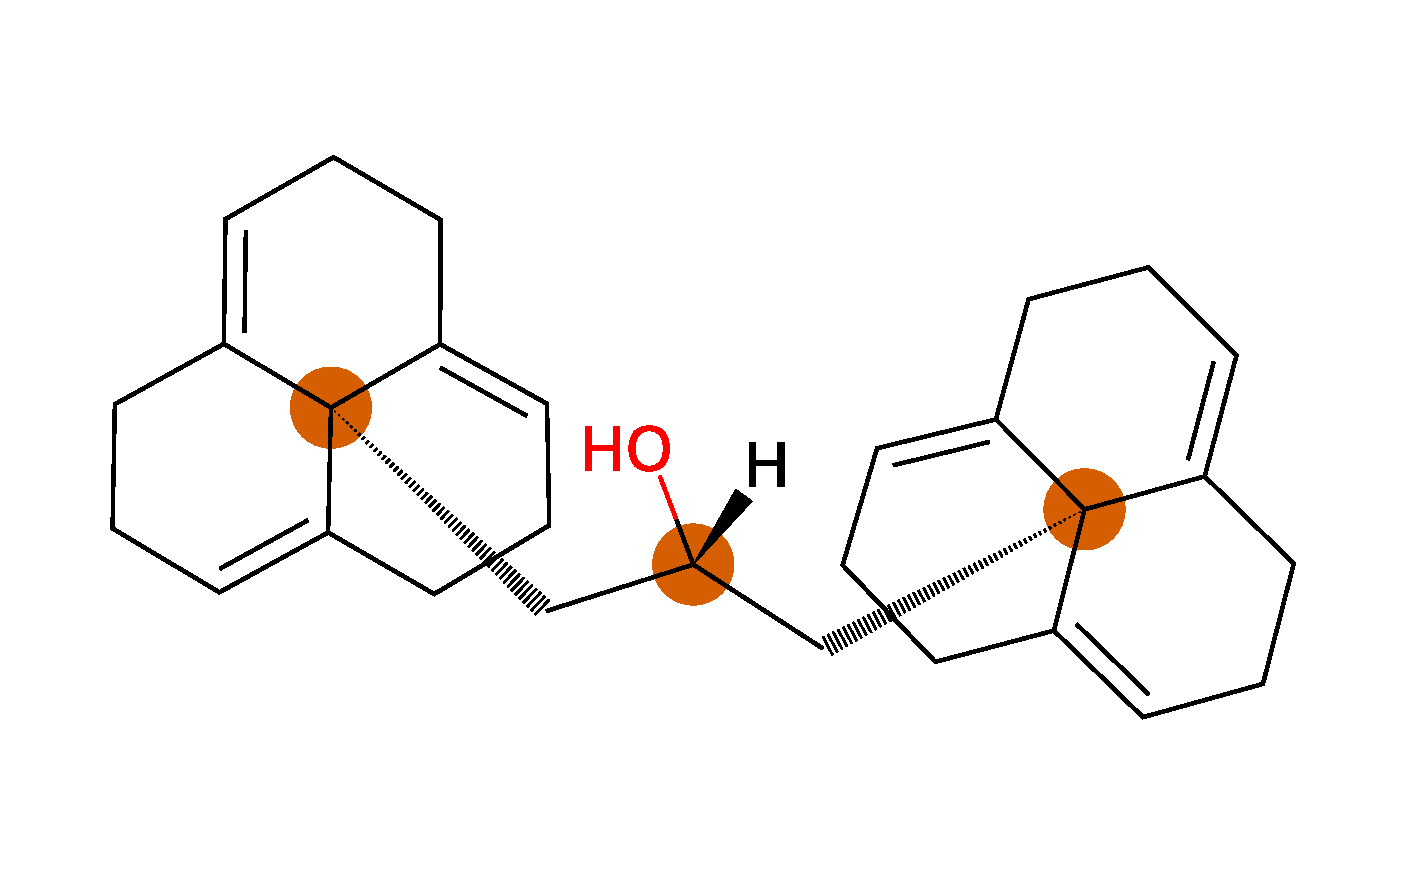
\includegraphics[width=6.0cm]{fig/exact_mirror_vs300.pdf}};
  \iosub{0.48,5.26}{D}{VS300}
  \node[acs,     anchor=east] at (3.55,0.55) {ACS topology: chiral};
  \node[achiral, anchor=west] at (3.85,0.55) {exact: achiral};
  \node[crit] at (3.70,0.05)
    {\(C_{\mathrm{SG}}(\mathcal X)=C_{\mathrm{SG}}(\mu\mathcal X)\)};
  \node[why] at (3.70,-0.43)
    {\(\mu\) fixes the center, exchanges the cages};
\end{scope}
\end{tikzpicture}
